
\chapter{Medición de erosión en un modelo físico de laboratorio}

\section{Descripción del modelo}

Los ensayos que se llevaron a cabo en este trabajo se realizaron en un modelo físico ubicado en el Laboratorio de Hidráulica de la Facultad de Ciencias Exactas, Físicas y Naturales (UNC). El modelo es una representación del Dique Los Molinos a escala reducida de longitudes 1:65. Este Dique se encuentra ubicado en la provincia Jujuy, sobre el río Grande, aguas debajo de la confluencia con el río Reyes. \\
Este modelo físico hidráulico está representado con fondo fijo en las márgenes y fondo móvil en el lecho del río. Se representaron las obras de regulación, con todos sus componentes y elementos auxiliares de relevancia hidrosedimentológica. Cuenta con un tramo del curso fluvial con un desarrollo total de aproximadamente 1520 m (1000 m aguas arriba y 520 m aguas abajo del dique), y un ancho efectivo variable entre los 250 m a 700 m en prototipo. Estas características permiten analizar adecuadamente el comportamiento hidrosedimentológico del flujo en cercanías de las obras, el funcionamiento de las operaciones de maniobra y la erosión en el tramo de río aguas abajo del dique. \\
Como se observa en la figura \ref{fig:modelo-fisico-dique-los-molinos}, el dique está constituido por un terraplén de materiales sueltos y dos vertederos, un tramo a nivel fijo (dique fijo), y otro regulado por 4 compuertas, conocido como dique móvil. Sobre margen derecha, se encuentra el canal moderador.

\begin{figure}[ht]
\centering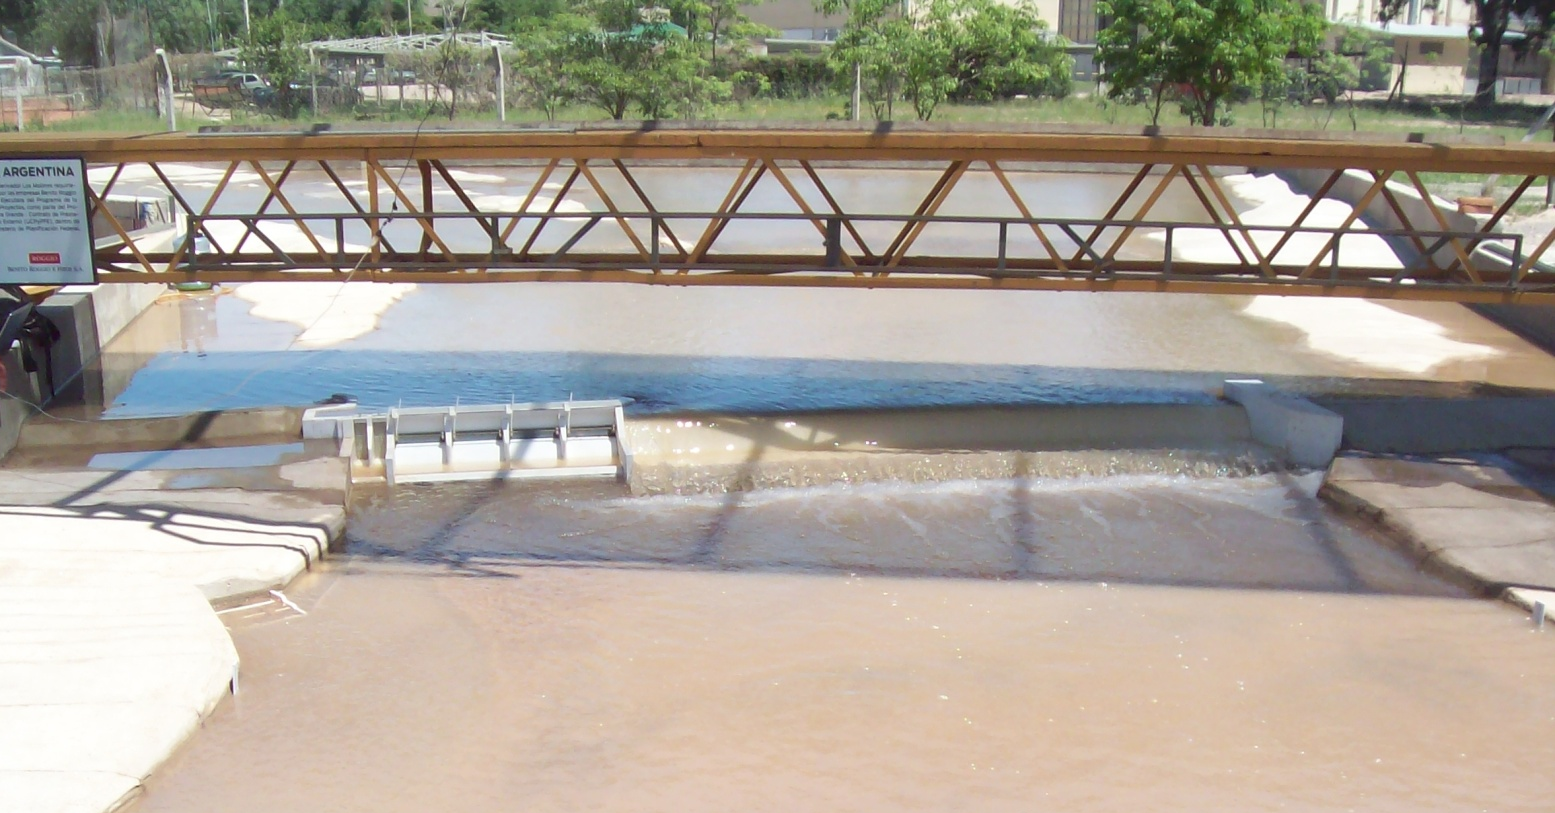
\includegraphics[width=\imsizeS]
{modelo-fisico-dique-los-molinos}
\caption[Modelo físico dique Los Molinos]{Modelo físico dique Los Molinos, Laboratorio de Hidráulica, FCEFyN de la UNC.}
\label{fig:modelo-fisico-dique-los-molinos}
\end{figure}

\begin{figure}[ht]

\centering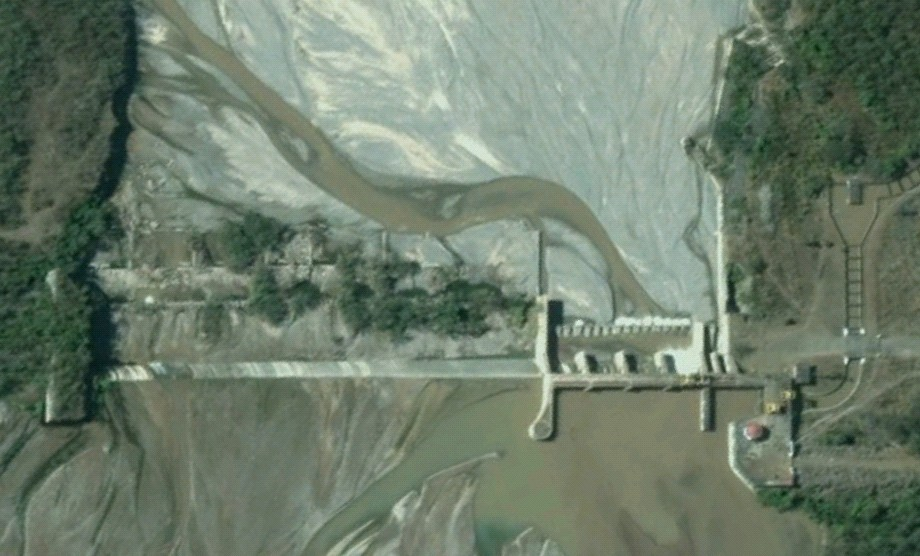
\includegraphics[width=\imsizeS]
{dique-los-molinos}
\caption[Dique Los Molinos]{Dique Los Molinos, Jujuy.}
\label{fig:dique-los-molinos}

\end{figure}

Teniendo en cuenta el alcance de este trabajo, los objetivos para el estudio sobre este modelo fueron:
\begin{itemize}

\item Analizar y cuantificar las erosiones locales, aguas abajo de las estructuras de descarga a los fines de constatar el funcionamiento de las obras previstas en el proyecto. Esta evaluación se llevará a cabo para escenarios hidrológicos de diseño.

\item Verificar y optimizar las consignas de operación de las estructuras de control, a los fines de regular los procesos hidrosedimentológicos frente a crecientes aguas arriba del dique móvil.

\end{itemize}

Sobre la zona relevante, se ha construido una plataforma móvil que posibilita realizar las mediciones de erosión. Figura \ref{fig:sistema-camara-carro}. Sus componentes principales son :

\begin{itemize}

\item Un puente grúa. Este puede ser trasladado para observar distintas áreas del modelo.

\item Una guia-riel y un carro-soporte para la cámara Kinect. La guía se anexa al puente grua, lo que permite la traslación de la cámara a lo ancho del modelo.

\end{itemize}

\begin{figure}[ht]
\centering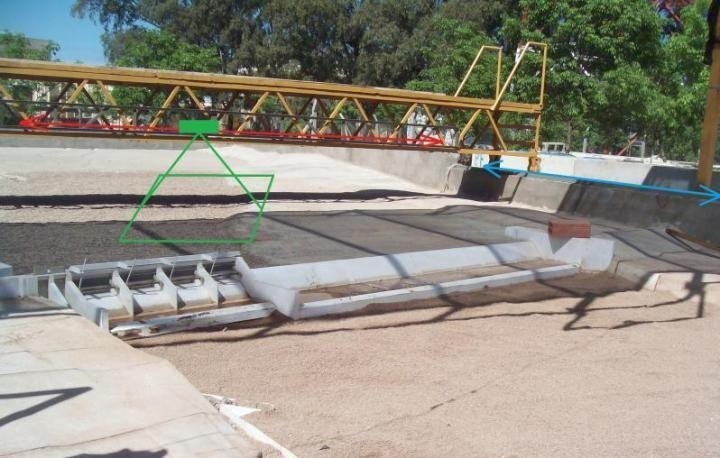
\includegraphics[width=\imsize]
{esquema-camara-puente-grua}
\caption[Puente grua]{Puente grua. Las flechas indican la direcciones en la que se puede trasladar la cámara (esquematizada con el recuadro verde). En rojo, traslación utilizando el carro soporte, mientras que la trayectoria en azul, se consigue movilizando el puente grúa.}
\label{fig:esquema-camara-puente-grua}
\end{figure}

\begin{figure}[ht]
\centering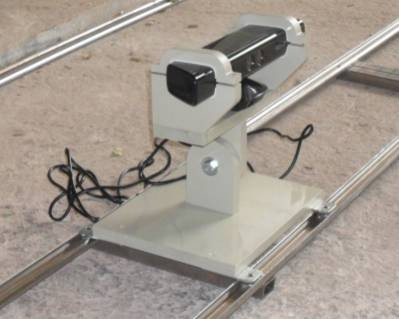
\includegraphics[width=\imsizeS]
{sistema-camara-carro}
\caption[Sistema cámara-soporte]{Soporte construido para trasladar la cámara sobre el modelo.}
\label{fig:sistema-camara-carro}
\end{figure}

%%%%%%%%%%%%%%%%%%%%%%%%%%%%%%%%%%%%%%%%%%%%%%%%%%%%%%%%%%%%%%%%%%%%%%%%%%%%%%%

\section{Etapas de un ensayo hidráulico}
\label{sec:etapas-previas-medicion}

En cada ensayo hidráulico realizado, se cubrieron las siguientes etapas :  
\begin{enumerate}

\item Se estableció la condición inicial del modelo, aguas abajo de las estructuras, nivelando el material suelto (arena) hasta la cota del terreno medido con la topografía provista. Figura \ref{fig:condicion-inicial-modelo}. Se utilizó una cota media de 1360 m s.n.m.

\item Encendido del modelo. Se encienden las bombas hidráulicas y comienza a recircular el agua dentro de cisternas y canales de aforos del laboratorio. Se realiza un manejo del sistema de bombeo hasta alcanzar el caudal establecido para cada  ensayo o escenario a simular.

\item Monitoreo de la erosión durante cada ensayo hasta alcanzar la condición de estabilidad. Estas mediciones se llevan a cabo con nivel óptico y mira. Se realizan mediciones de nivel en las zonas de interés durante intervalos temporales regulares, hasta medir valores similares entre estos intervalos.

\item Apagado del modelo. Se apagan las bombas hidráulicas, se cierran las compuertas correspondientes, y se deja drenar el modelo.

\item Medición de erosión. Esta etapa se desarrollará en detalle en las siguientes secciones.

\end{enumerate}

\begin{figure}[ht]
\centering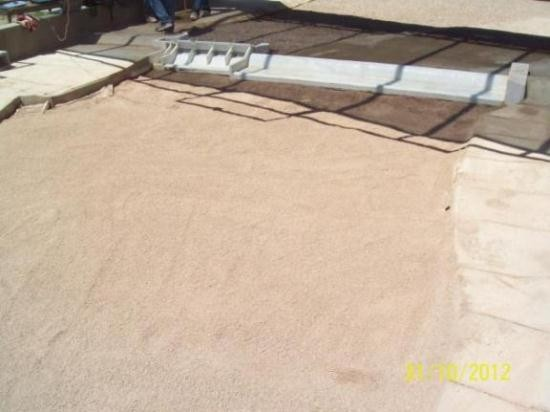
\includegraphics[width=\imsizeS]
{condicion-inicial-modelo}
\caption[Condición inicial del modelo]
{Condición inicial del modelo}
\label{fig:condicion-inicial-modelo}
\end{figure}

%%%%%%%%%%%%%%%%%%%%%%%%%%%%%%%%%%%%%%%%%%%%%%%%%%%%%%%%%%%%%%%%%%%%%%%%%%%%%%%

\section{Metodología de medición con nivel óptico}

La técnica tradicional consiste en el relevamiento manual de puntos sobre perfiles longitudinales y transversales (en la figura \ref{fig:esquema-perfiles}), por lo general cada 10 cm, utilizando para dicha tarea el nivel óptico (en la figura \ref{fig:nivel-optico}) y una mira con una escala graduada al milímetro.  

\begin{figure}[ht]
\centering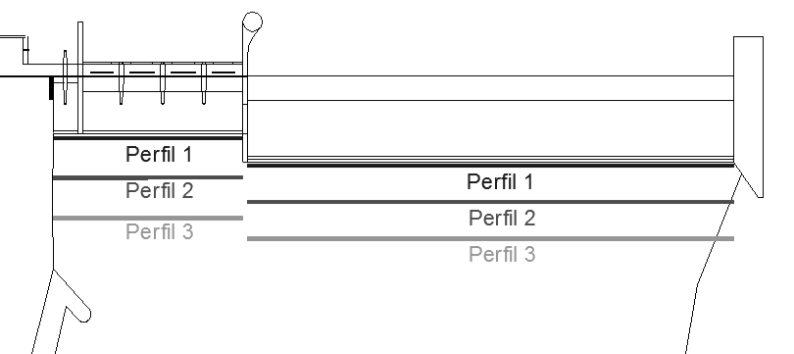
\includegraphics[width=\imsize]
{esquema-perfiles}
\caption[Perfiles transversales]
{Ubicación de perfiles transversales para medir las erosiones finales.}
\label{fig:esquema-perfiles}
\end{figure}

\begin{figure}[ht]
\centering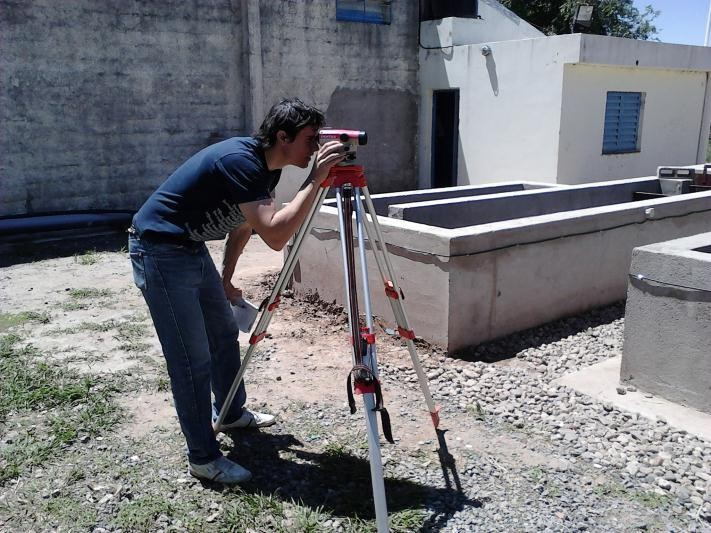
\includegraphics[width=\imsize]
{nivel-optico}
\caption[Nivel óptico]
{Medición con nivel óptico en modelo físico Los Molinos, cortesía de Nicolás Bellino.}
\label{fig:nivel-optico}
\end{figure}

Por último, se realiza la digitalización manual y conversión de modelo a prototipo de los puntos relevados.

\section{Metodología de medición con la cámara RGB-D}
\label{sec:metodologia-medicion-digital}

En esta sección, se describe la aplicación de la técnica digital de medición de erosión propuesta en este trabajo. \\

Se tuvieron en cuenta un conjunto de consideraciones que forman parte de la técnica de medición y permiten obtener resultados óptimos, estas consideraciones son las siguientes :

\begin{itemize}

\item La superficie a relevar debe estar libre de agua. Como se mencionó en \ref{sec:consideraciones-kinect}, se observó que los objetos con características reflectantes afectan al sensor de profundidad de la Kinect. Figura \ref{fig:modelo-condiciones-agua}.

\item La escena debe estar al resguardo de la luz solar, como se explica en \ref{sec:consideraciones-kinect}. Debido a que el modelo físico utilizado se encontraba al aire libre, en el exterior del Laboratorio de Hidráulica, fue necesario utilizar un nylon de color negro colocado sobre el puente grúa, como se puede observar en la figura \ref{fig:modelo-lona}. Alternativamente, se considero realizar las mediciones al atardecer cuando la luz solar es más tenue. Se concluye que utilizando el nylon se obtienen condiciones lumínicas estables, quitando así una restricción para el horario de medición.

\item La guía debe estar horizontalizada. El plano desde el que se captura la escena debe estar a una altitud constante para que la representación de la superficie sea consistente. Esta condición debe ser verificada al iniciar cada ensayo hidráulico.

\item La cámara debe ubicarse en un rango de 0.4 m  a 1.5 m de altura sobre escena a relevar, para que el error de medición se mantenga dentro del intervalo aceptable (aproximadamente 5 mm), segun el analisis del sensor Kinect presentado en \ref{sec:consideraciones-kinect}.

\end{itemize}

\begin{figure}[h]
\centering
\begin{minipage}[t]{.45\textwidth}
\begin{center}
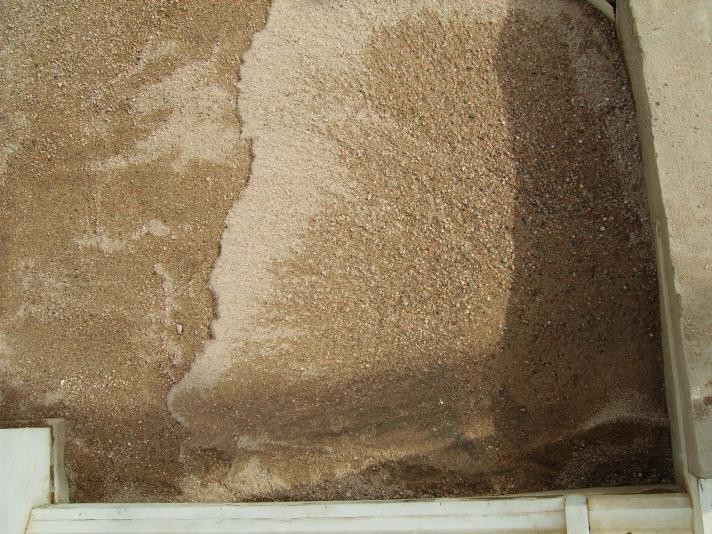
\includegraphics[width=\imsizeS]{modelo-sin-agua} % primera imagen colocada a la izquierda
\end{center}
\end{minipage}
\hfill
\begin{minipage}[t]{.45\textwidth}
\begin{center}
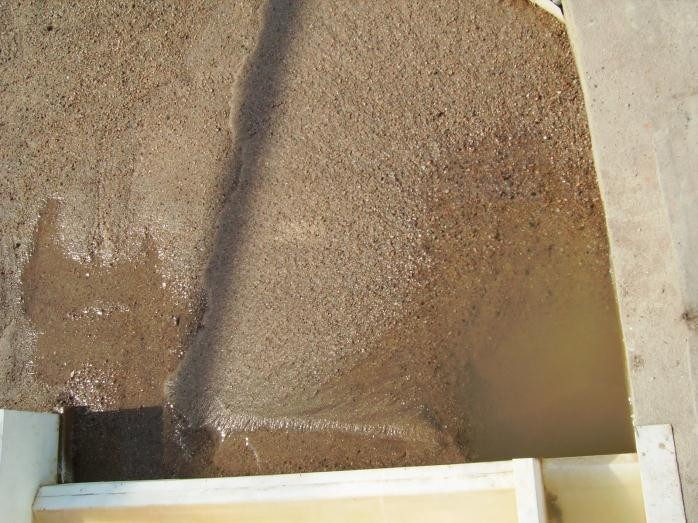
\includegraphics[width=\imsizeS]{modelo-con-agua} % segunda imagen colocada a la derecha
\end{center}
\end{minipage}
\hfill
\caption{A la derecha condición correcta para la medición. A la izquierda se observan espejos de agua que interfieren el sensor infrarrojo de la cámara.}
\label{fig:modelo-condiciones-agua}
\end{figure}

\begin{figure}[h]
\centering
\begin{minipage}[t]{.45\textwidth}
\begin{center}
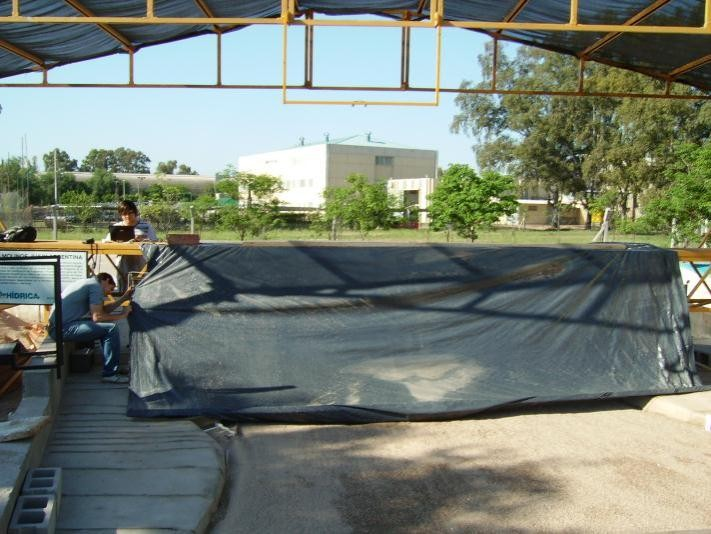
\includegraphics[width=\imsizeS]{modelo-lona1} % primera imagen colocada a la izquierda
\end{center}
\end{minipage}
\hfill
\begin{minipage}[t]{.45\textwidth}
\begin{center}
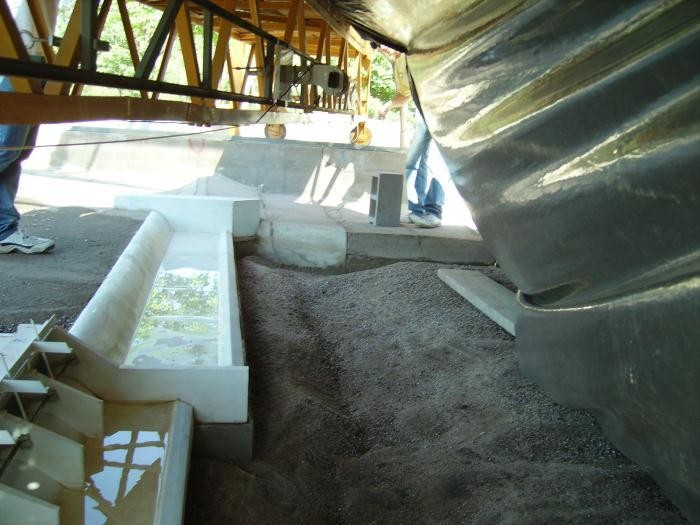
\includegraphics[width=\imsizeS]{modelo-lona2} % segunda imagen colocada a la derecha
\end{center}
\end{minipage}
\hfill
\caption{Derecha: Forma de colocar el nylon sobre el puente grúa para cubrir todo el largo del riel. Izquierda: La sombra producida por el nylon permite capturar las imágenes sin interferencia del sol.}
\label{fig:modelo-lona}
\end{figure}

Habiendo verificado las condiciones anteriores, se introduce el carro-soporte en carril guía y se inicia la aplicación de registración \textit{ModelMapper} \ref{sec:model-mapper}. \\
 
En la figura \ref{fig:aguas-abajo-desplazamiento-carro}, se observa cómo manipular la plataforma móvil para capturar la escena. Se propone un desplazamiento del carro de aproximadamente 40 cm entre cada captura, para que el área sobrelapada entre dos nubes puntos continuas esté próxima al 50\%. Si la aplicación no lograr realizar la registración correctamente se corrige la ubicación del sensor a una posición intermedia.

\begin{figure}[ht]
\centering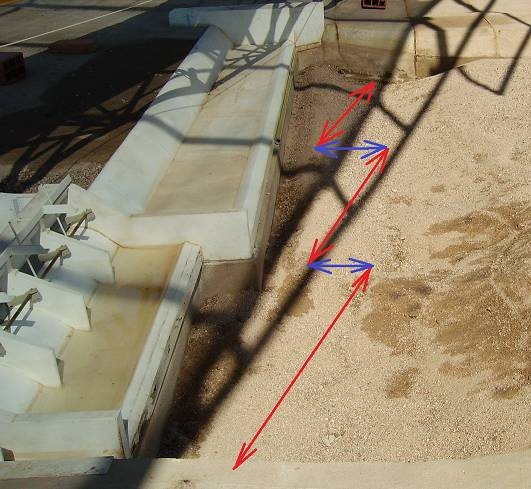
\includegraphics[width=\imsize]
{aguas-abajo-desplazamiento-carro}
\caption[Desplazamiento de la cámara]{Recorrido del puente grúa y del carro-soporte sobre la escena. Las flechas rojas indican desplazamiento de la cámara y las flechas azules representan el movimiento del puente.}
\label{fig:aguas-abajo-desplazamiento-carro}
\end{figure}

En el apartado \ref{sec:conversion-mapa3D-prototipo} se describe que para realizar la conversión a prototipo es necesario un punto fijo con cotas conocidas en los sistemas del modelo y del prototipo. Con este fin, se recomienda que la escena capture las estructuras fijas en el modelo físico con medidas de elevación dada por mediciones topográficas. En caso contrario, se puede medir con nivel óptico un punto visible en la escena y utilizar su cota prototipo como referencia.  

%%%%%%%%%%%%%%%%%%%%%%%%%%%%%%%%%%%%%%%%%%%%%%%%%%%%%%%%%%%%%%%%%%%%%%%%%%%%%%%

\section{Ensayos realizados}
En la tabla siguiente se presenta un resumen de los ensayos realizados. Se detallan los caudales asociados así como las estructuras hidráulicas por las que pasa cada uno y su representatividad.\\

\begin{tabular}{ccc}
\hline
Ensayo  & Caudal total $m^{3}/s$ & Motivación \\
\hline
1 & 900 & Caudal Máximo Dique Móvil (DM) y \\
  &     & Canal Moderador (CM) \\
\hline
2 & 3200 & Caudal Máximo Sólo Dique Fijo (DF) \\
\hline
3,7,9 & 4200 & Caudal para Periodo de Retorno T=10000 años \\
\hline
4 & 90 & Caudal de Despegue CM \\
\hline
5 & 225 & Caudal de Despegue DM \\
\hline
10 & 600 & Caudal de Verificación DF, DM y CM
 \\
\hline
13 & 1600 & Caudal de Verificación DF, DM y CM
 \\
\hline
14 & 600 & Caudal de Verificación DM y CM
 \\
\hline
\end{tabular}

\newpage % Salto de página para acomodar las imágenes

\subsection{Medición de erosión máxima}
\label{sec:ensayo-erosion-maxima}

En el ámbito de la Ingeniería Civil, la representación con modelos físicos a escala reducida y la simulación de ensayos hidráulicos fluviales, como los que aquí se presentan, tiene entre sus objetivos principales definir las cotas de erosión máxima. Estas mediciones se realizan con el fin de establecer las profundidades de fundación de los muros de contención de las estructuras hidráulicas que componen el sistema evaluado. \\
Se muestran los mapas de elevación en escala prototipo, generados a partir del relevamiento de fosos de erosión ubicados aguas abajo de las estructuras, para los ensayos 1 y 3. Como punto de referencia se utilizó la parte superior del dique móvil, con cota igual a 1377.77 m s.n.m.\\

\begin{figure}[h]
\centering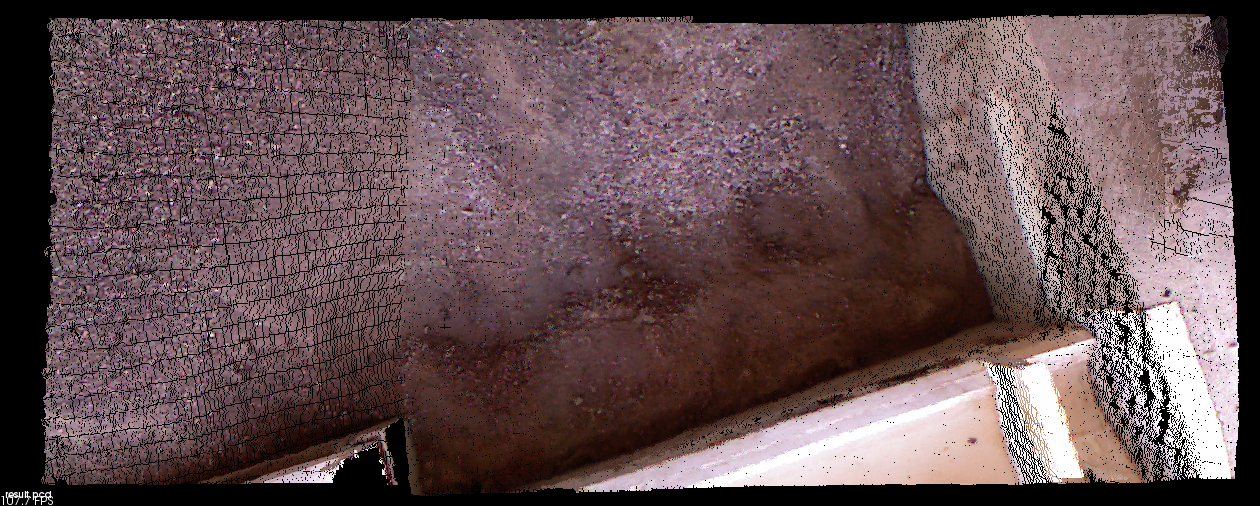
\includegraphics[width=\imsizeL]
{fosos_erosion_Q900_rgb}
\caption[Imagen RGB Ensayo 1]
{Ensayo 1. Foso de erosión aguas abajo del dique móvil.  Imagen RGB.}
\label{fig:fosos_erosion_Q900_rgb}
\end{figure}

\begin{figure}[h]
\centering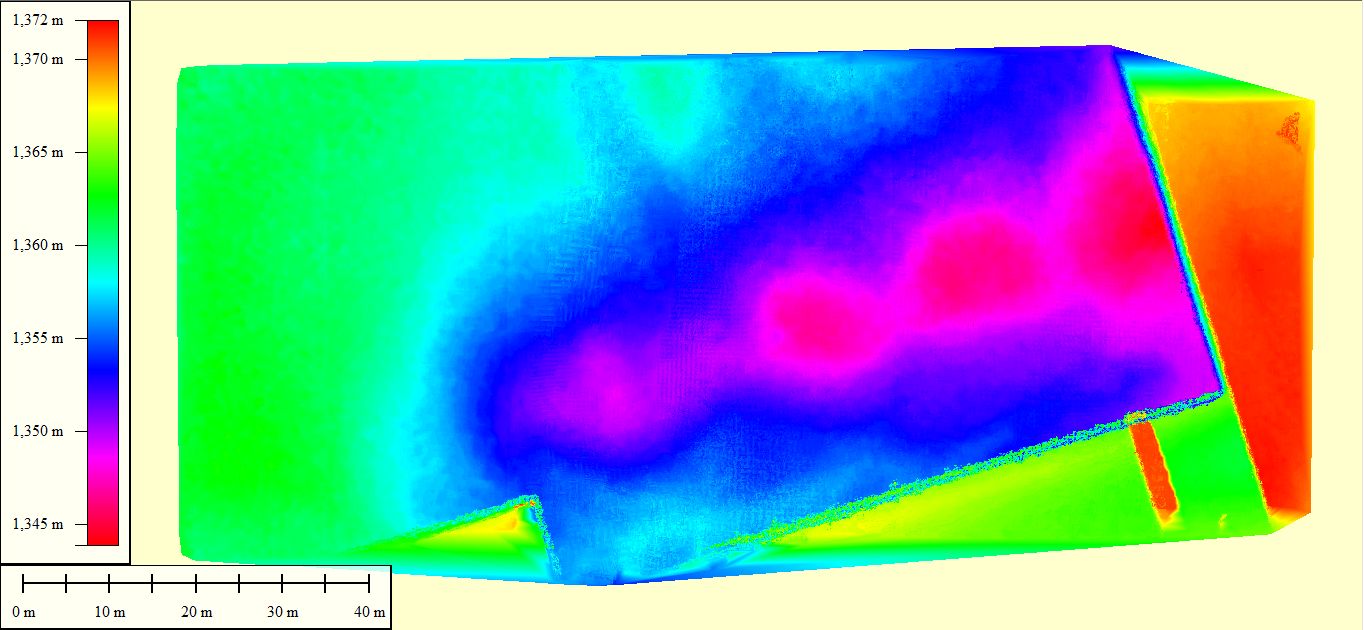
\includegraphics[width=\imsizeL]
{Q900_dem}
\caption[DEM Ensayo 1]
{Ensayo 1. Foso de erosión aguas abajo del dique móvil. Modelo digital de elevaciones (DEM).}
\label{fig:Q900_dem}
\end{figure}

\begin{figure}[h]
\centering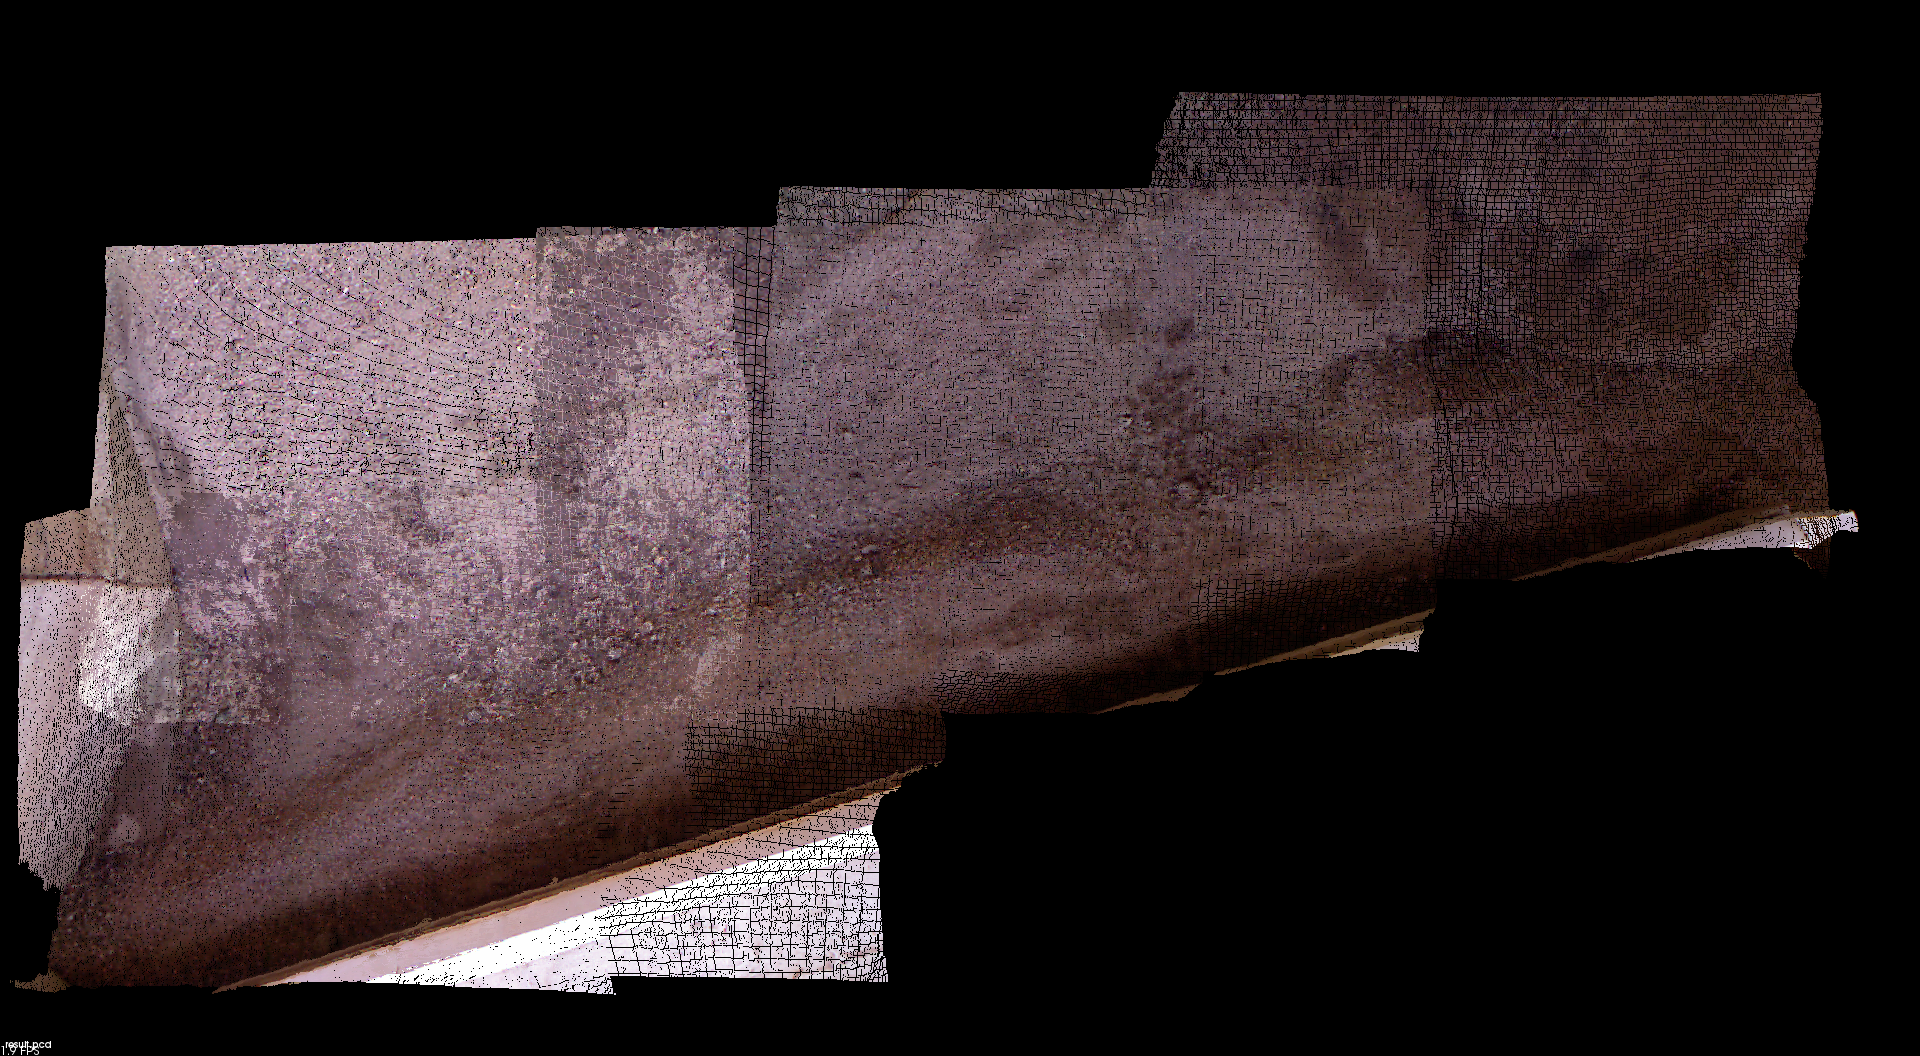
\includegraphics[width=\imsizeL]
{Q4200_rgb}
\caption[Imagen RGB Ensayo 3]
{Ensayo 3. Foso de erosión aguas abajo del dique fijo. Imagen RGB.}
\label{fig:Q4200_rgb}
\end{figure}

\begin{figure}[h]
\centering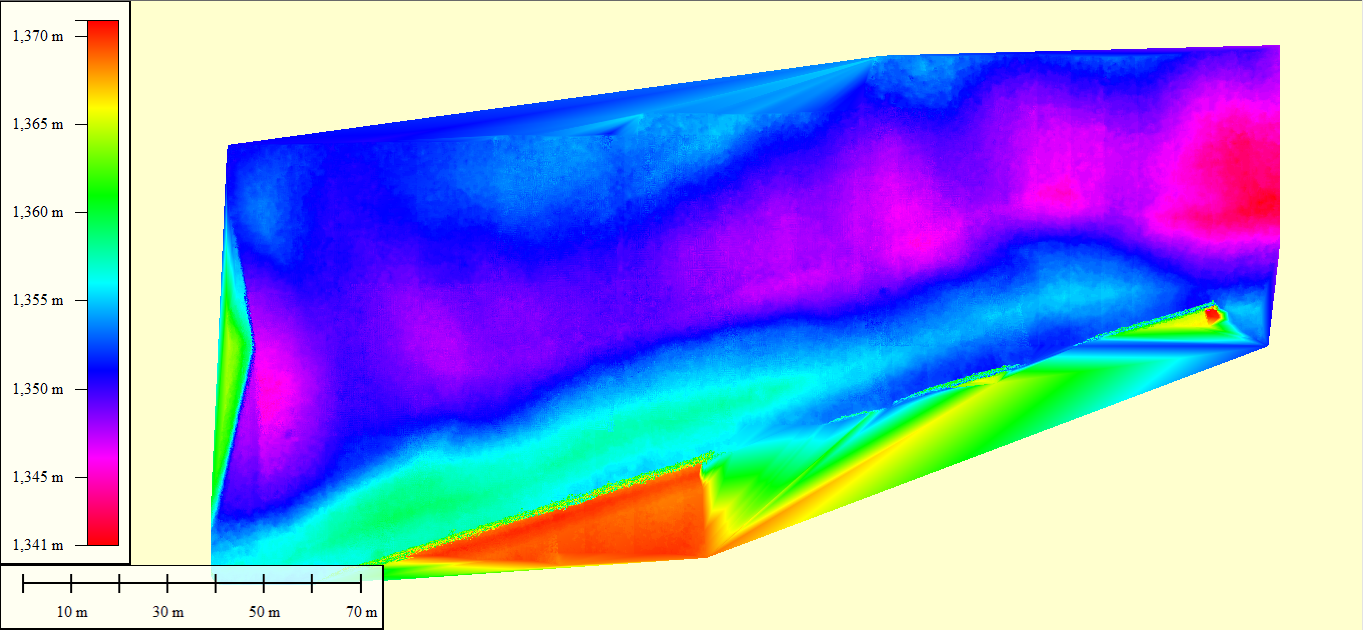
\includegraphics[width=\imsizeL]
{Q4200_dem}
\caption[DEM Ensayo 3]
{Ensayo 1. Foso de erosión aguas abajo del dique fijo. Modelo digital de elevaciones.}
\label{fig:Q4200_dem}
\end{figure}

\subsection{Medición de formas de fondo}
\label{sec:ensayo-formas-de-fondo}

Estas mediciones se realizaron con el objetivo de verificar y optimizar las consignas de operación de las estructuras de control, con el fin de regular los procesos hidrosedimentológicos presentes en las proximidades de la presa aguas arriba.\\
En este ensayo se relevaron las canalizaciones hacia las compuertas del dique móvil y el canal moderador. El análisis de los canales que se formaron sobre la superficie del modelo, debido a las llamadas que se realiza con la operación de las estructuras de control, requiere relevar una densidad de puntos elevada y a la vez cubrir grandes áreas de superficie. La técnica digital aborda esta tarea de forma mucha más eficiente y precisa que la metodología tradicional. \\
Se muestran los mapas de elevación en escala prototipo, generados a partir del área de modelación aguas arriba del dique, para el ensayo 10. Como punto de referencia se utilizó la parte superior del dique móvil, con cota igual a 1377.77 m s.n.m.

\begin{figure}[ht]
\centering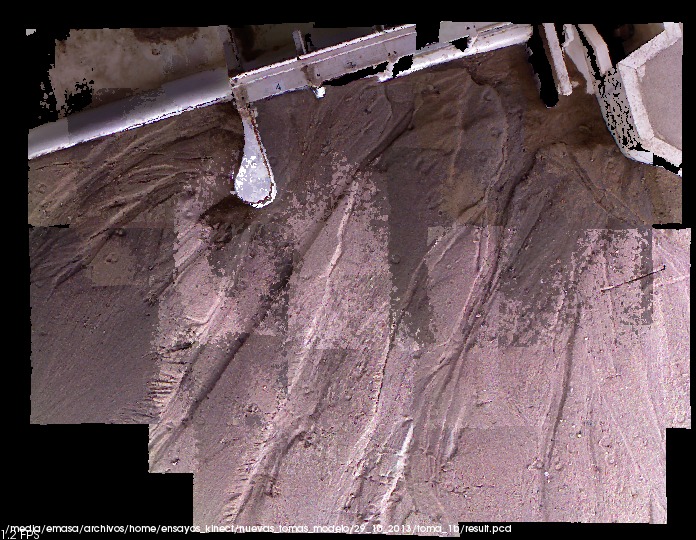
\includegraphics[width=\imsize]
{Q600_rgb}
\caption[Imagen RGB Ensayo 10]
{Ensayo 10. Área aguas arriba del dique móvil. Imagen RGB.}
\label{fig:Q600_rgb}
\end{figure}

\begin{figure}[ht]
\centering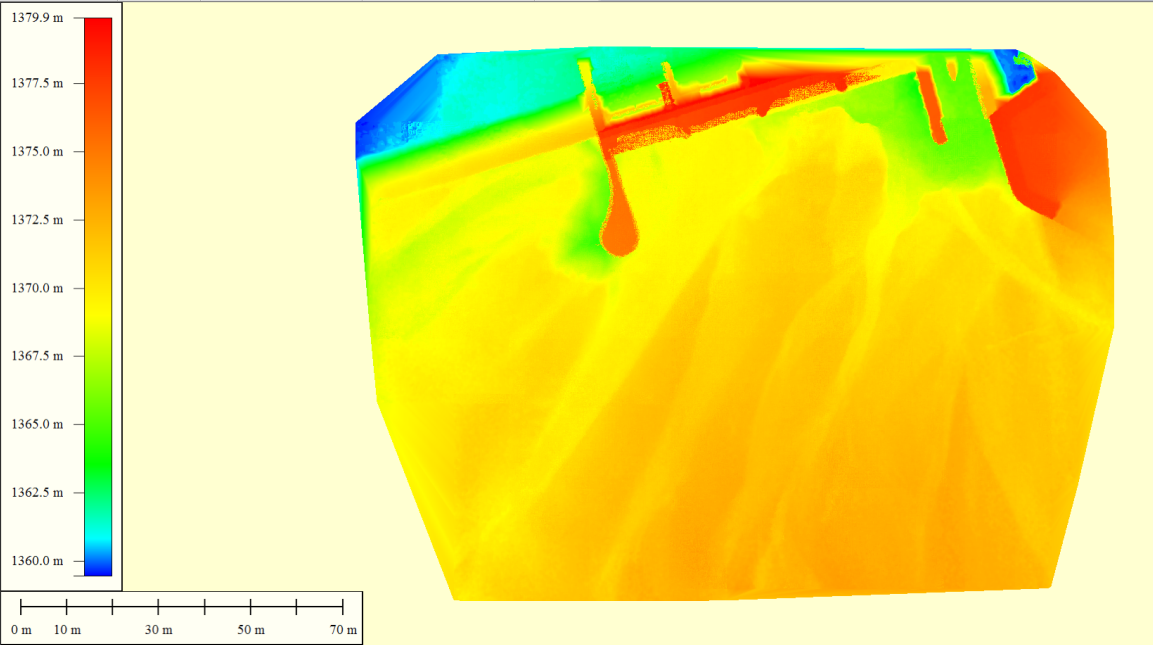
\includegraphics[width=\imsizeL]
{Q600_dem}
\caption[DEM Ensayo 10]
{Ensayo 10. Área aguas arriba del dique móvil. Modelo digital de elevaciones.}
\label{fig:Q600_dem}
\end{figure}

